\section{Set 集合}

\begin{Java}
public interface Set<E> extends Collection<E>
\end{Java}

Set 接口继承自 Collection 接口,新增的方法和 List 类似。

Set 的默认实现类 AbstractSet 实现了三个方法:

\begin{Java}
// 判断相等,需要调用 containsAll 方法
public boolean equals(Object o)
// 获取哈希码
public int hashCode()
// 移除所有元素,需要调用 remove 方法
public boolean removeAll(Collection<?> c)
\end{Java}

Set 的主要子类继承关系如下:

\begin{center}
    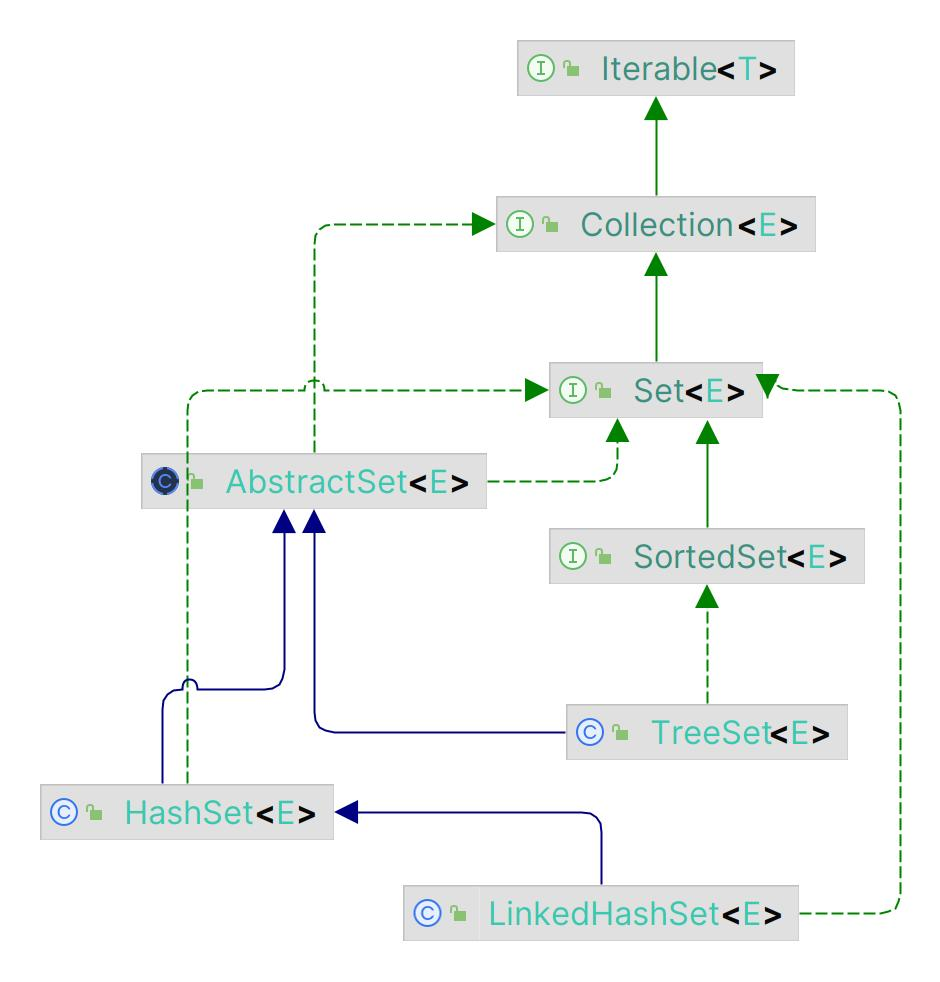
\includegraphics[width=0.5\linewidth]{../../../imgs/Set.jpg}
\end{center}

可以发现,Set 的几个实现类和 Map 存在对应关系,因为 Set 的底层就是用 Map 进行存储。会了 Map 基本就会了 Set。这节只讲个 HashSet,其他两个自行理解。

\subsection{HashSet}

HashSet 底层使用 HashMap 存储数据,本质上是对 HashMap 的封装以及 Set 功能的实现:

\begin{Java}
public class HashSet<E> extends AbstractSet<E> implements Set<E>, Cloneable, java.io.Serializable
\end{Java}

HashSet 有两个关键的成员:

\begin{Java}
private transient HashMap<E,Object> map;
private static final Object PRESENT = new Object();
\end{Java}

这个 PRESENT 是干什么的呢,我们知道,Map.Entry 必须具有四个属性: hashCode, key, value, next。其中 KV 用于存储键值对,但是 SET 是单个元素的容器,因此,KV 只能留一个,而要留也只能留 K,所以我们必须找个东西填充 V,这个东西就是 PRESENT。因此前面加了 static final 进行优化。

这样我们就能很好地理解 HashSet 实现 SET 功能的原理了: K-V 对中,K必须是唯一的,V 全是相同的一个对象。到这里,HashSet 就讲完了,它的所有特性都和 HashMap 一致。

\begin{Java}
public boolean add(E e) {
    return map.put(e, PRESENT)==null;
}
public boolean remove(Object o) {
    return map.remove(o)==PRESENT;
}
\end{Java}

\newpage